 \documentclass[12pt, dvipdfmx]{beamer}

\renewcommand{\kanjifamilydefault}{\gtdefault}
%%%%%%%%%%%  package  %%%%%%%%%%%
\usepackage{bxdpx-beamer}% dvipdfmxなので必要
\usepackage{pxjahyper}% 日本語で'しおり'したい

\usepackage{amssymb,amsmath,ascmac}

\usepackage{multirow}
\usepackage{bm}

\graphicspath{{../../_Figures//}{../../_Figures/Rheology/}}

\usepackage{tikz}
\usepackage{xparse}

\usepackage{multimedia}

\usetikzlibrary{shapes,arrows}
%% define fancy arrow. \tikzfancyarrow[<option>]{<text>}. ex: \tikzfancyarrow[fill=red!5]{hoge}
\tikzset{arrowstyle/.style n args={2}{inner ysep=0.1ex, inner xsep=0.5em, minimum height=2em, draw=#2, fill=black!20, font=\sffamily\bfseries, single arrow, single arrow head extend=0.4em, #1,}}
\NewDocumentCommand{\tikzfancyarrow}{O{fill=black!20} O{none}  m}{
\tikz[baseline=-0.5ex]\node [arrowstyle={#1}{#2}] {#3 \mathstrut};}

%目次スライド
\AtBeginSection[]{
  \frame{\tableofcontents[currentsection]}
}

%アペンディックスのページ番号除去
\newcommand{\backupbegin}{
   \newcounter{framenumberappendix}
   \setcounter{framenumberappendix}{\value{framenumber}}
}
\newcommand{\backupend}{
   \addtocounter{framenumberappendix}{-\value{framenumber}}
   \addtocounter{framenumber}{\value{framenumberappendix}} 
}

\newcommand{\rmd}{\mathrm{d}}
\newcommand{\dd}[1]{\dfrac{\mathrm{d} #1}{\mathrm{d} x}}

%%%%%%%%%%%  theme  %%%%%%%%%%%
\usetheme{Copenhagen}
% \usetheme{Metropolis}
% \usetheme{CambridgeUS}
% \usetheme{Berlin}

%%%%%%%%%%%  inner theme  %%%%%%%%%%%
% \useinnertheme{default}

% %%%%%%%%%%%  outer theme  %%%%%%%%%%%
\useoutertheme{default}
% \useoutertheme{infolines}

%%%%%%%%%%%  color theme  %%%%%%%%%%%
%\usecolortheme{structure}

%%%%%%%%%%%  font theme  %%%%%%%%%%%
\usefonttheme{professionalfonts}
%\usefonttheme{default}

%%%%%%%%%%%  degree of transparency  %%%%%%%%%%%
%\setbeamercovered{transparent=30}

% \setbeamertemplate{items}[default]

%%%%%%%%%%%  numbering  %%%%%%%%%%%
% \setbeamertemplate{numbered}
\setbeamertemplate{navigation symbols}{}
\setbeamertemplate{footline}[frame number]


\title
[複雑な事象について]
{複雑な事象について}
\author[東亞合成 佐々木]{佐々木 裕}
\institute[東亞合成]{東亞合成株式会社}
\date{\today}

\begin{document}

%%%%%
% 1 P
%%%%%
\maketitle

%%%%%
% 2 P
%%%%%
%% 目次 (必要なければ省略)
\begin{frame}
\frametitle{Outline}
\tableofcontents
\end{frame}

\begin{frame}
	\frametitle{この章でのお話}


	% 具体的に列記すると、以下のような事項となります。
	\begin{itemize}
		\item 流れるということについて、もう少し
		\begin{itemize}
			\item 
		\end{itemize} 
		\item 非ニュートン流体
		\begin{itemize}
			\item 
		\end{itemize} 
		\item 固体についても、もう少し
		\begin{itemize}
			\item 
		\end{itemize}
	\end{itemize}
\end{frame}

\section{流れるということについて、もう少し}

\subsection{ニュートン流体を見直しましょう}
\begin{frame}
    \frametitle{ニュートンの法則}
		\begin{columns}[T, onlytextwidth]
			\column{.48\linewidth}
				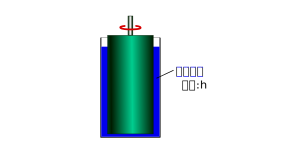
\includegraphics[width=.7\textwidth]{nijyu_entou.png}
			\column{.48\linewidth}
				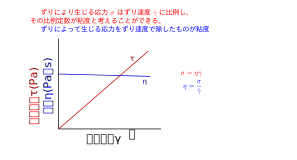
\includegraphics[width=.9\textwidth]{newtonian.png}
		\end{columns}
		\begin{exampleblock}{ニュートンの法則}
			\vspace{-5mm}
			\begin{align*}
				\text{せん断応力} &= \text{比例定数} \times \text{せん断速度} \notag \\
				\tau = \eta \dot{\gamma}
			\end{align*}
			% \vspace{-4mm}
			\textcolor{red}{比例定数が、物質の流れ易さを表す「粘度」 $\eta$}
		\end{exampleblock}
\end{frame}

\begin{frame}
	\frametitle{液体の流動を表すモデル}
	\begin{block}{液体を考えるときに重要な事項}
		\begin{itemize}
			\item \textcolor{red}{固体と接している液体はその相対的な移動速度が同じ}
			\begin{itemize}
				\item 移動する板と接している層 0 は\textcolor{red}{板と同じ速度 $v$ で流れ、}
				\item \textcolor{red}{地面に接している層 $n$ は流れない。}
			\end{itemize}
		\end{itemize}
	\end{block}
	\begin{exampleblock}{水面に板を浮かべたモデル}
		\begin{columns}[T, onlytextwidth]
			\column{.65\linewidth}
				\begin{itemize}
					\item 水深方向に n+1 層に分割
						\begin{itemize}
							\item 水面の板との境目を0
							\item 水底との境目を n 
						\end{itemize}
						\item 液体の内部では、
						\begin{itemize}
							\item 水深に応じて流れる速度の分布
							\item 最も単純な状態:\\速度勾配が一定
						\end{itemize}
				\end{itemize}
			\column{.32\linewidth}
				\begin{center}
					\includegraphics[width=.9\textwidth]{shear_3.png}
				\end{center}
		\end{columns}
	\end{exampleblock}
\end{frame}

\begin{frame}
	\frametitle{液体の流動について}
		\begin{itemize}
			\item 評価の対象である液体の内部では、
			\begin{itemize}
				\item 水深に応じて、流れる速度の分布が生じる
			\end{itemize}
			\item 液体の流れる速度は、
			\begin{itemize}
				\item 水深 $y$ の関数として $v(y)$
				\item 速度勾配と呼ばれ、その単位は $[\mathrm{s^{-1}}]$
			\end{itemize}
		\end{itemize}
		\begin{screen}
			速度勾配は、せん断変形を記述する無次元量であるせん断ひずみ $\gamma$ の時間変化(微分)$\Leftrightarrow$ せん断速度
			\begin{align*}
				\dfrac{\mathrm{d} v}{\mathrm{d} y} =\dot{\gamma} [s^{-1}]
			\end{align*}
		\end{screen}
\end{frame}

\begin{frame}
	\frametitle{液体の力学モデル}
	\vspace{-3mm}
		\begin{columns}[c, onlytextwidth]
			\column{.48\linewidth}
				\begin{itemize}
					\item せん断速度$\dot{\gamma}$ に比例し、
					\item せん断応力 $\tau$ が生じ、
					\item 比例定数が粘度 $\eta$
				\end{itemize}
				\vspace{-2mm}
				\begin{align*}
					\tau = \eta \dot{\gamma}
				\end{align*}
				\vspace{-6mm}
				\begin{screen}
					上記の比例関係が成立する液体がニュートン流体
				\end{screen}
			\column{.48\linewidth}
				\begin{center}
					\includegraphics[width=\textwidth]{shear_4.png}
				\end{center}
		\end{columns}
		\begin{alertblock}{注意点}
			\begin{itemize}
				\item 速度勾配に従って、各層ごとにせん断応力が発生
				\item その値は、\alert{局所的なせん断速度に比例して変化。}
				\item 逆に言えば、\alert{せん断速度によらずに粘度が一定。}
			\end{itemize}
		\end{alertblock}
\end{frame}

\begin{frame}
	\frametitle{液体の応力とは?(再掲)}
		\begin{itemize}
			\item マクロな変形(例えば、ずり変形)を付与
			\begin{itemize}
				\item ミクロにも粒子近傍が変形
			\end{itemize}
			\item 一粒子に着目すると、
			\begin{itemize}
				\item その粒子を取り巻く周りの粒子とのポテンシャル場が変化して、\textcolor{red}{「歪んだかご」}
				\item 「歪んだかご」の中で、\textcolor{red}{居心地が悪くなる。}
				\item その結果として\textcolor{red}{局所的な応力が発現}
			\end{itemize}
			\item その積分値として、マクロな応力
			\begin{itemize}
				\item 「歪んだかご」からの\alert{脱出 $\Leftrightarrow$ ミクロな応力が消失 }
				\item マクロにも\alert{流動}
			\end{itemize}
		\end{itemize}
		\vspace{3mm}
		\begin{center}
			\includegraphics[width=.6\textwidth]{liquid_flow.png}
		\end{center}
\end{frame}

\begin{frame}
	\frametitle{ニュートン流体の粘度が「せん断速度」に\\依存しない理由}
		\vspace{-3mm}
		\begin{columns}[T, onlytextwidth]
			\column{.48\linewidth}
				\begin{block}{せん断応力の由来}
					\begin{itemize}
						\item 仮想的な面で生じる\\せん断応力の由来は、
						\begin{itemize}
							\item \alert{面を通しての粒子の相互作用}に起因
							\item 相対的な速度差に、比例する
						\end{itemize}
						\item この相互作用は、
						\begin{itemize}
							\item 「歪んだかご」からの脱出頻度にも比例
							\item 多体の相互作用が、「居心地の悪さ」
						\end{itemize}
					\end{itemize}
				\end{block}
			\column{.48\linewidth}
				\vspace{3mm}
				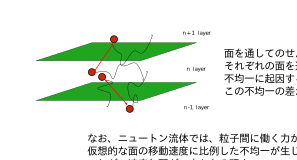
\includegraphics[width=\textwidth]{flow_layer.png}
				\begin{exampleblock}{ニュートン流体では}
					\begin{itemize}
						\item 隣接する粒子間の相互作用が、\alert{せん断速度やせん断応力に非依存。}
						\item 結果、粘度が一定。
						\item ただし、\alert{適正な範囲で。}
					\end{itemize}
				\end{exampleblock}
		\end{columns}
\end{frame}

\begin{frame}
    \frametitle{少しだけ大粒子が入った場合}
		\begin{itemize}
			\item ニュートン流体に球状粒子が入った場合。
				\begin{itemize}
					\item アインシュタインが理論的に導出
					\item 剛直な球を希薄に懸濁した溶液
				\end{itemize}
			\item 仮定条件
				\begin{itemize}
					\item 球の半径は、液体粒子より遥かに大きい。
					\item 球状粒子間の相互作用はない。
					\item 液体粒子は球状粒子に固着している。
				\end{itemize}
			\item 下式を使って、砂糖分子の大きさと分子数を概算
		\end{itemize}
		\begin{block}{アインシュタインの粘度式}
			\vspace{-5mm}
			\begin{align*}
				&\eta = \eta_0(1+2.5\phi) \\
				&\text{ただし、$\eta_0$は液体の粘度、} \\
				&\text{$\phi$ は球状粒子の体積分率}
			\end{align*}
		\end{block}
\end{frame}

\subsection{時間と温度との関係}
\begin{frame}
	\frametitle{時間と温度の関係を議論するために}
		ここでは、粘弾性現象における「時間と温度の関係」を議論するために必要となるアイテムの整理を行おう。
		\begin{itemize}
			\item 「時間と温度の関係」を議論するときに、統計力学的な考え方が有効となる
			\footnote{
				その導出過程の議論は省略して、天下りに議論します。
			}。
			\item その要点
			\begin{itemize}
				\item 微視的に見た粒子は、平均として $k_BT$ 程度のエネルギー
				\footnote{
					``$k_B$'' は、ボルツマン定数と呼ばれ、その単位は JK$^{-1}$
				}を持っている。\\
			ただし、\alert{あくまでも平均であることに注意。}
				\item 微視的な状態の生じやすさをボルツマン統計で議論できるとする。
			\end{itemize}
		\end{itemize}
		% \begin{itemize}
		% 	\item かごの正体は、互いの粒子が相互作用した結果
		% 	\item 結局、この微視的状態のエネルギーも粒子と同程度の平均 
		% \end{itemize}
\end{frame}

\begin{frame}
	\frametitle{液体の応力とは?}
		\begin{itemize}
			\item マクロな変形(例えば、ずり変形)を付与
			\begin{itemize}
				\item ミクロにも粒子近傍が変形
			\end{itemize}
			\item 一粒子に着目すると、
			\begin{itemize}
				\item その粒子を取り巻く周りの粒子とのポテンシャル場が変化して、\textcolor{red}{「歪んだかご」}
				\item 「歪んだかご」の中で、\textcolor{red}{居心地が悪くなる。}
				\item その結果として\textcolor{red}{局所的な応力が発現}
			\end{itemize}
			\item その積分値として、マクロな応力
			\begin{itemize}
				\item 「歪んだかご」からの\alert{脱出 $\Leftrightarrow$ ミクロな応力が消失 }
				\item マクロにも\alert{流動}
			\end{itemize}
		\end{itemize}
		\vspace{3mm}
		\begin{center}
			\includegraphics[width=.6\textwidth]{liquid_flow.png}
		\end{center}
\end{frame}

\section{非ニュートン流体}

\subsection{身近な液体とその分類}
\begin{frame}
	\frametitle{身近な液体}
		\begin{center}
			\includegraphics[width=.7\textwidth]{viscosity.jpg}

        \href{https://www.iwakipumps.jp/blog/naruhodo/08/}{この絵のサイトへのリンク}
		\end{center}
\end{frame}

\begin{frame}
	\frametitle{各種の応答特性の分類}
		\begin{itemize}
			\item 図の左側が弾性応答
			\item 右側が流動特性
			\item 単純に二分されるわけでもなく、粘性と弾性を\\併せ持ったものが多く存在。
		\end{itemize}
			\includegraphics[width=\textwidth]{reoroji.jpeg}
			Nature 1942 v149-3790, p702
			% \href{http://rheology.jp/nagoya/2017/10/%e3%83%ac%e3%82%aa%e3%83%ad%e3%82%b8%e3%83%bc%e7%9a%84%e3%81%aa%e7%89%a9%e8%b3%aa%e3%81%ae%e5%88%86%e9%a1%9e/}{この絵のサイトへのリンク}
\end{frame}


\subsection{不均一のある流体}
\begin{frame}
	\frametitle{<title>}
		\begin{columns}[T, onlytextwidth]
			\column{.48\linewidth}
				\includegraphics[width=\textwidth]{flow.png}
			\column{.48\linewidth}
				\includegraphics[width=\textwidth]{particle.png}
		\end{columns}
\end{frame}

\section{固体についても、もう少し}
\subsection{固体と液体の境目についても}
\begin{frame}
    \frametitle{固体と液体の境目}
    \begin{itemize}
        \item 現象論的な理解
            \begin{itemize}
                \item 熱エネルギーの大小で変化
                \item 変形速度(時間の進み方)でも変わる。
            \end{itemize}
        \item ポイント
            \begin{itemize}
                \item 境目は曖昧
                \item 時間と温度の関係が大事⇔粘弾性
                \item 内部構造の有無が大事
            \end{itemize}
    \end{itemize}
\end{frame}

\begin{frame}
    \frametitle{熱力学的に考えると}
    自由エネルギー
    
    相転移の判断基準

    自由エネルギーについて

\end{frame}

\begin{frame}
    \frametitle{結晶化とガラス転移}
        \begin{itemize}
            \item 結晶化:粒子同士が規則的に並ぶ
            \item ガラス化:液体と類似の状態で動けなくなる。
                \begin{itemize}
                    \item 二次の相転移⇔転移熱は発生しない
                \end{itemize}
        \end{itemize}


        \begin{itemize}
            \item 液体と固体の境目は、はなはだ曖昧。
                \begin{itemize}
                    \item 特に固体が結晶ではないとき。
                    \item ガラス状態を液体と見分けるのは難しい。
                \end{itemize}
            \item 高分子では、
                \begin{itemize}
                    \item 部分的に液体なので、両面性を有する。
                    \item 粘弾性が重要。
                \end{itemize}
        \end{itemize}
\end{frame}

\subsection{金属の強さと弱さ}
\begin{frame}
	\frametitle{(おまけ)金属の強さと弱さ}
		\begin{columns}[T, onlytextwidth]
			\column{.48\linewidth}
				\begin{itemize}
					\item イオン結合ではミクロなズレが生じにくい
					\item 金属ではずり変形も可能
				\end{itemize}
				\begin{center}
					\includegraphics[width=\textwidth]{kinzoku_ion.png}
				\end{center}
				
			\column{.48\linewidth}
				\begin{itemize}
					\item 欠損の存在が変形時の応力を低減
				\end{itemize}
				\begin{center}
					\includegraphics[width=\textwidth]{kinzoku_henkei.png}
				\end{center}
		\end{columns}
	\href{https://www.hik.shiga-irc.go.jp/info/instructions/metal/metal2/}{これらの図のサイトへのリンク}
\end{frame}


% \appendix
% \backupbegin

% % \section{演習問題 1}
% % \subsection{「物質の三態について」}
% % \begin{frame}
% % 	\frametitle{「物質の三態について」}
% % 	\scriptsize
% % 	以下の穴を埋めてください。
% % 		\begin{itemize}
% % 			\item 関数の役割を考えてみると、\fbox{\textcolor{red}{入力}}を変換装置に入れた結果として\fbox{\textcolor{red}{出力}}が現れるわけですから、入力と出力との間の\fbox{\textcolor{red}{関係}}を表していると考えることもできます。
% % 			\item また、関数というのは、\fbox{\textcolor{red}{数の集合}}に値を取る\fbox{\textcolor{red}{写像}}の一種と考えることもできます。
% % 			\item グラフとは、\fbox{\textcolor{red}{入力}}と\fbox{\textcolor{red}{出力}}との関係を\fbox{\textcolor{red}{平面図}}に示したものであり、視覚的にその関係を理解しやすくしたものと考えることができます。
% % 			\item このグラフに表した関数の\fbox{\textcolor{red}{形}}を見ることで、入力と出力との\fbox{\textcolor{red}{関係}}を直感的に理解することができます。
% % 		\end{itemize}
% % \end{frame}

% \backupend
\end{document}